%%%%%%%%%%%%%%%%%%%%%%%%%%%%%%%%%%%%%%%%%%%%%%%%%%%
%
%  New template code for TAMU Theses and Dissertations starting Fall 2016.
%
%
%  Original Author: Sean Zachary Roberson
%  This version adapted for URS by Parasol lab.
%  Adapted from version 3.16.10, which was last updated on 9/29/2016.
%  URS adaptation last updated 1/9/2017.
%
%%%%%%%%%%%%%%%%%%%%%%%%%%%%%%%%%%%%%%%%%%%%%%%%%%%
%%%%%%%%%%%%%%%%%%%%%%%%%%%%%%%%%%%%%%%%%%%%%%%%%%%%%%%%%%%%%%%%%%%%%%
%%                           SECTION III
%%%%%%%%%%%%%%%%%%%%%%%%%%%%%%%%%%%%%%%%%%%%%%%%%%%%%%%%%%%%%%%%%%%%%

\chapter{THE IMPLEMENTATION}

\section{The Textbook}

For the implementation of the design, I have gone with proof of concept model. The textbook that will first be integrated with my adviser's Mathematics textbook.

\section{Textbook Build Process}

Talk about the JSON hierarchy that the textbook depends on

\section{The Tech Stack}

Give basic high level overview of the application on how a user interacts with it

\section{Integration with Textbook}

How the json is imported into application then exported for use by the textbook

% \section{}
% \begin{figure}[h!]
% 	\centering
% 	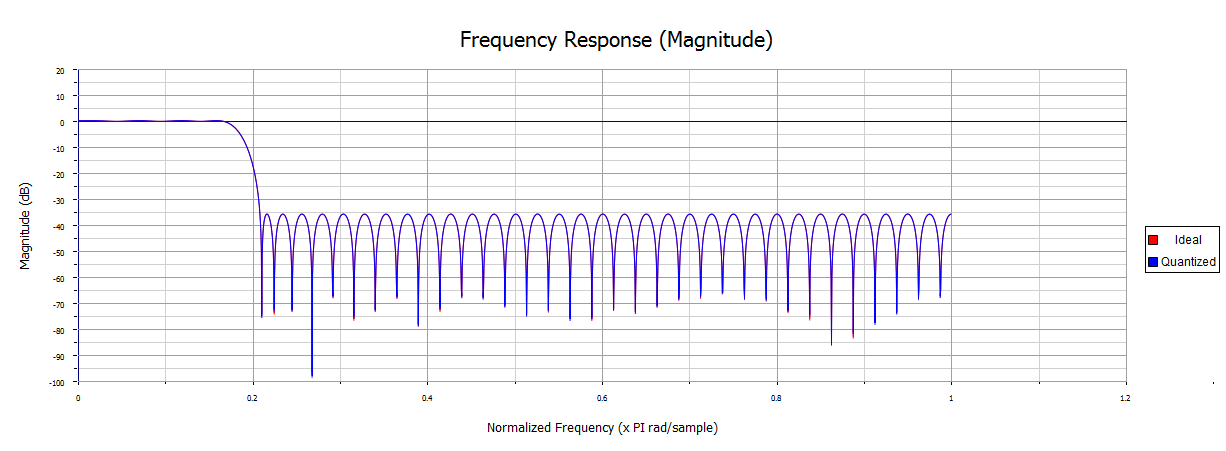
\includegraphics[scale=0.5]{LowPass_Filter_Design.png}
% 	\caption{A low pass filter design.}
% \end{figure}
